\documentclass[10pt,a4paper]{article}

%----------------------------------------------------------------------------------------
%	PACKAGES AND THEMES
%----------------------------------------------------------------------------------------
\usepackage[utf8]{inputenc}
\usepackage[T1]{fontenc}
\usepackage[sc]{mathpazo} % Palatino
\linespread{1.05}

\usepackage{graphicx}
\usepackage{tikz} % circular photo
\usepackage[margin=0.5in, top=0.5in]{geometry}
\usepackage[usenames,dvipsnames]{xcolor}
\usepackage{hyperref}
\usepackage{enumitem}
\usepackage{titlesec}
\usepackage{ragged2e}
\usepackage{fontawesome5}
\usepackage{tabularx}
\usepackage{needspace}

% COLORS: deep teal, matched to the website
\definecolor{Accent}{RGB}{15, 64, 72}
\definecolor{Muted}{RGB}{80, 96, 100}

\hypersetup{
    colorlinks=true,
    linkcolor=Accent,
    urlcolor=Accent,
    pdftitle={Soinik Ghosh - CV},
    pdfauthor={Soinik Ghosh},
}

\titleformat{\section}{
  \vspace{-6pt}\scshape\raggedright\large\bfseries\color{Accent}
}{}{0em}{}[\color{Accent}\titlerule \vspace{-4pt}]

\setlist[itemize]{leftmargin=*, noitemsep, topsep=2pt, parsep=2pt}

% \entry{Institution}{Place}{Role or degree}{Dates}
\newcommand{\entry}[4]{
  \noindent\textbf{#1} \hfill \textit{#2} \\
  \textit{#3} \hfill #4 \par
  \vspace{3pt}
}

% \project{Title}{Context}{Description}
\newcommand{\project}[3]{
  \noindent\textbf{#1} \hfill \textit{\small #2} \\
  {\small #3} \par
  \vspace{4pt}
}

\newcommand{\me}{\textbf{S.~Ghosh}}

\begin{document}
\pagestyle{empty}

%----------------------------------------------------------------------------------------
%	HEADER
%----------------------------------------------------------------------------------------
\noindent
\begin{minipage}[c]{0.18\textwidth}
    \begin{tikzpicture}
        \clip (0,0) circle (1.25cm);
        \node at (0,0) {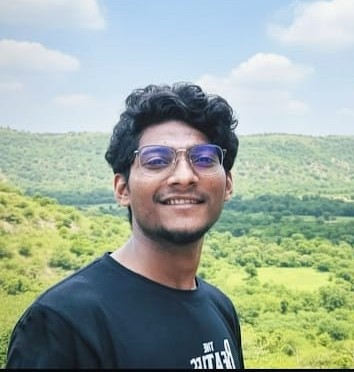
\includegraphics[width=2.5cm]{profile-photo.jpeg}};
    \end{tikzpicture}
\end{minipage}
\hfill
\begin{minipage}[c]{0.78\textwidth}
    {\fontsize{28pt}{28pt}\selectfont\scshape\bfseries\color{Accent} Soinik Ghosh} \\[4pt]
    {\large PhD Researcher, Biomedical Engineering \textbullet{} Co-Founder, Hridae Medical Technologies} \\[6pt]

    \small
    \faMapMarker* School of Biomedical Engineering, IIT (BHU) Varanasi \textbar{} Kolkata, India \\
    \faPhone* (+91) 98756 81292 \textbar{}
    \faEnvelope[regular]~\href{mailto:soinikghosh.rs.bme23@itbhu.ac.in}{soinikghosh.rs.bme23@itbhu.ac.in} \textbar{}
    \href{mailto:soinikghosh9@gmail.com}{soinikghosh9@gmail.com}\\
    \faGlobe~\href{https://soinikghosh9.github.io/personal-website/}{soinikghosh9.github.io/personal-website} \textbar{}
    \faBook~\href{https://scholar.google.com/citations?user=l9U73kcAAAAJ&hl=en}{Google Scholar} \textbar{}
    \faOrcid~\href{https://orcid.org/0009-0000-8277-8710}{0009-0000-8277-8710} \\
    \faGithub~\href{https://github.com/soinikghosh9}{github.com/soinikghosh9} \textbar{}
    \faLinkedin~\href{https://www.linkedin.com/in/soinik-ghosh-103411270}{linkedin.com/in/soinik-ghosh-103411270}
\end{minipage}

\vspace{10pt}

%----------------------------------------------------------------------------------------
%	RESEARCH PROFILE
%----------------------------------------------------------------------------------------
\section{Research Profile}
\small
PhD researcher in biomedical engineering working on AI for clinical neurophysiology and medical imaging. My doctoral research develops EEG-based screening, triage and decision-support tools for dementia and epilepsy, with an emphasis on interpretable signal features and testing on independent clinical cohorts. This includes first-author work on reduced-electrode EEG for cognitive screening, accepted at GlobalSouthAI @ NeurIPS 2026, and on patient-adaptive seizure detection, published in Computers in Biology and Medicine. I also build automated medical imaging pipelines and lightweight AI agents that run locally. As a co-founder of Hridae Medical Technologies, I work on wearable monitoring and ECG models for precision cardiology and neurology. I trained in physiology and neuroscience before moving into engineering.

\vspace{8pt}

%----------------------------------------------------------------------------------------
%	EDUCATION
%----------------------------------------------------------------------------------------
\section{Education}
\entry{Indian Institute of Technology (BHU) Varanasi}{Varanasi, India}{PhD in Biomedical Engineering (CGPA: 9.6/10)}{07/2023 -- Present}
\footnotesize \textit{Thesis area: EEG-based screening, triage and clinical decision support.}

\entry{University of Calcutta}{Kolkata, India}{M.Sc in Physiology (Neuroscience specialisation), First Class (CGPA: 7.4/10)}{09/2019 -- 09/2021}
\footnotesize \textit{Thesis: ``Neuropsychophysiological Behaviour of Adenosine: Crosstalks between Neurotransmitters''}

\entry{Surendranath College, University of Calcutta}{Kolkata, India}{B.Sc in Human Physiology (Honours)}{07/2016 -- 06/2019}

\vspace{8pt}

%----------------------------------------------------------------------------------------
%	POSITIONS
%----------------------------------------------------------------------------------------
\section{Positions}
\project{Co-Founder, Hridae Medical Technologies Pvt. Ltd.}{01/2026 -- Present}
{Wearable monitoring for precision cardiology and neurology: devices, ECG and other analysis models, and clinician review software, developed with clinicians.}

\project{Doctoral Researcher \& Teaching Assistant, School of Biomedical Engineering, IIT (BHU)}{07/2023 -- Present}
{EEG-based screening and triage tools and clinical decision-support systems, with a focus on interpretability and testing on independent cohorts. In collaboration with the Department of Neurology, IMS BHU, and with AIIMS New Delhi, IIT Kanpur and IIT Kharagpur. Experimental design, data collection and analysis, algorithm development, scientific writing and teaching.}

\vspace{8pt}

%----------------------------------------------------------------------------------------
%	PUBLICATIONS
%----------------------------------------------------------------------------------------
\section{Publications}
\textit{\small Published and accepted work only. Full list on \href{https://scholar.google.com/citations?user=l9U73kcAAAAJ&hl=en}{Google Scholar}.}

\vspace{2pt}
\noindent\textbf{\small Journal articles}
\begin{itemize}
    \item \me, S.~Sharma, N.~Sharma. \href{https://doi.org/10.1016/j.compbiomed.2025.111398}{\textit{GenEEG: Improving epileptic EEG detection through patient-adaptive latent diffusion and continual learning.}} Computers in Biology and Medicine, vol.~201, 111398 (2026).
\end{itemize}

\noindent\textbf{\small Book chapters}
\begin{itemize}
    \item \me, F.~Yasmeen, S.~Sharma, N.~Sharma. \href{https://doi.org/10.1007/978-3-032-20634-3_28}{\textit{Decoding the neural dynamics of motor imagery and execution: an EEG-based investigation into conscious hand movement representation.}} In: Cognitive Biomarkers and BCI Applications, Proceedings of MBCC 2025, Springer, 2026, pp.~311--322.
    \item F.~Yasmeen, \me, P.~Jangra, N.~Sharma, S.~Sharma. \href{https://doi.org/10.1007/978-3-032-20634-3_21}{\textit{ME-GSE: an end-to-end classification of motor imagery EEG signals using graph-based spectral embedding.}} In: Cognitive Biomarkers and BCI Applications, Proceedings of MBCC 2025, Springer, 2026.
\end{itemize}

\noindent\textbf{\small Workshop and conference papers}
\begin{itemize}
    \item \me, R.~N.~Chaurasia, S.~Sharma, N.~Sharma. \textit{Decomposing a clinical EEG montage for low-channel cognitive triage: placement, age referencing and output design.} GlobalSouthAI Workshop @ NeurIPS 2026, Sydney (accepted). \href{https://github.com/soinikghosh9/lowchannel-eeg-triage}{[code]}
    \item \href{https://doi.org/10.1109/ICCSAI64074.2025.11064720}{\textit{A hybrid classical-quantum model for enhanced MRI-based brain tumor classification using transfer learning and quantum neural networks.}} IEEE ICCSAI 2025 (co-author).
    \item \me, C.~Parikshith, F.~Yasmeen, A.~K.~Srivastava, S.~Sharma, N.~Sharma. \href{https://doi.org/10.1109/AKGEC62572.2024.10868917}{\textit{Real-time brain signals monitoring system using single-channel EEG for BCI applications.}} IEEE AKGEC 2024.
    \item P.~Chavakula, \me, N.~Sharma, D.~Kumar. \href{https://doi.org/10.1109/INSPECT63485.2024.10896072}{\textit{Development of a haptic exo-suit with tactile feedback in hand rehabilitation.}} IEEE INSPECT 2024.
\end{itemize}

\vspace{6pt}

%----------------------------------------------------------------------------------------
%	FEATURED RESEARCH
%----------------------------------------------------------------------------------------
\section{Featured Research}
\project{Low-channel EEG for cognitive triage}{GlobalSouthAI @ NeurIPS 2026 \textbullet{} IIT (BHU), IMS BHU}
{Studied how far a clinical EEG can be simplified for cognitive screening, using memory-clinic recordings re-derived to simulate low-channel devices and independent cohorts from other hospitals. A few well-placed electrodes screened about as well as the full clinical montage, and EEG added value beyond age alone; detecting mild cognitive impairment remains an open problem. Proposes a simplified recording design for prospective device studies.}

%----------------------------------------------------------------------------------------
%	CURRENT RESEARCH
%----------------------------------------------------------------------------------------
\section{Current Research}
\begin{itemize}
    \item \textbf{Low-channel EEG screening for dementia:} electrode placement, sampling and output design for cognitive triage devices, tested at hospitals not used in training.
    \item \textbf{Epilepsy monitoring and seizure forecasting:} patient-adaptive EEG monitoring and probabilistic forecasting of seizure risk.
    \item \textbf{Wearable monitoring and ECG (Hridae):} wearable devices, ECG models and patient-specific heart models for precision cardiology and neurology.
    \item \textbf{Automated medical image processing:} automated pipelines that prepare and analyse images across medical imaging modalities.
    \item \textbf{Local AI agents:} lightweight agents on an 8 GB laptop GPU for coding, research and document work.
    \item \textbf{Offline cognitive assessment:} browser-based battery across eleven cognitive domains with on-device measures and within-person change tracking.
\end{itemize}

\vspace{6pt}

\vspace{6pt}

%----------------------------------------------------------------------------------------
%	SELECTED PROJECTS
%----------------------------------------------------------------------------------------
\section{Selected Projects}
\project{GenEEG: patient-adaptive synthetic EEG}{IIT (BHU)}
{Latent diffusion that generates synthetic seizure EEG, with continual learning one patient at a time. \href{https://github.com/soinikghosh9/GenEEG}{[code]}}

\project{Hridayam: AI-assisted non-invasive cardiovascular imaging}{Smart India Hackathon 2024, Winner}
{Multi-sensor, point-of-care cardiovascular screening prototype. \href{https://github.com/soinikghosh9/Hridayam}{[code]}}

\project{Firefly: VR-guided robotic exosuit for stroke rehabilitation}{PRAGATI Hackathon 2023, 2nd runner-up}
{VR environment coupled to a robotic exoskeleton. \href{https://github.com/soinikghosh9/Firefly}{[code]}}

\project{Motor-imagery BCI for prosthetic control}{IIT (BHU)}
{Translates motor-imagery EEG into prosthetic arm commands in real time, decoding live on a Raspberry Pi 5.}

\project{GemSAM: explainable multimodal image analysis on edge hardware}{Kaggle MedGemma Impact Challenge 2026}
{Agentic pipeline combining MedGemma and SAM~2. \href{https://github.com/soinikghosh9/GemSAM}{[code]}}

\project{CogniDhi and HippoSphere AI}{Stanford Longevity Design Challenge 2025--26; MIT Media Lab Moodeng AI Challenge}
{Cognitive health platform; lightweight computer vision for animal behaviour monitoring. \href{https://cogni-dhi.vercel.app/}{[CogniDhi]} \href{https://github.com/soinikghosh9/hipposphere-ai}{[HippoSphere]}}

\vspace{6pt}

%----------------------------------------------------------------------------------------
%	SKILLS
%----------------------------------------------------------------------------------------
\section{Skills}
\begin{tabularx}{\textwidth}{@{}l X@{}}
\textbf{Signals \& models:} & EEG, ECG and PCG processing; qEEG and spectral features; ICA artefact handling; source connectivity; GNNs; latent diffusion; continual and patient-adaptive learning; medical image processing; LLM-based agents \\
\textbf{Evaluation:} & Subject-grouped cross-validation; external-cohort testing; shortcut and confound checks; paired bootstrap and permutation tests; calibration \\
\textbf{Engineering:} & Python, PyTorch, MNE, MATLAB, C/C++, C\#, TypeScript, React, GCP; embedded EEG, low-noise PCB design, Raspberry Pi and microcontrollers; Unity VR/XR \\
\textbf{Clinical \& lab:} & Clinical study design and ethics applications; clinician review workflows; cell culture, molecular biology, animal studies \\
\end{tabularx}

\vspace{6pt}

%----------------------------------------------------------------------------------------
%	HONOURS & TRAINING
%----------------------------------------------------------------------------------------
\section{Honours \& Training}
\begin{itemize}
    \item \textbf{Winner}, Smart India Hackathon 2024 (Hardware Edition), Government of India.
    \item \textbf{2nd Runner-up}, PRAGATI Hackathon 2023, iHub Drishti (TIH), IIT Jodhpur.
    \item \textbf{GATE 2023}, Life Sciences, All India Rank 1313.
    \item g.tec BCI \& Neurotechnology Spring School 2025: invasive and non-invasive BCI.
    \item Neurogati / CNS Lab, IIT Madras: computational brain modelling and brain-inspired AI.
    \item SERB Karyashala, IIT Roorkee: AI in human brain-computer interaction.
    \item CSIR-IICB Skill Development Programme: molecular cloning, protein expression and characterisation.
\end{itemize}

\vspace{6pt}

%----------------------------------------------------------------------------------------
%	BEYOND SCIENCE
%----------------------------------------------------------------------------------------
\Needspace{2\baselineskip}
\section{Beyond Science}
\small
Independent artist, musician and filmmaker (\href{https://open.spotify.com/artist/3VprLdYpRRnk0ymHHozFOb/}{music}, \href{https://www.imdb.com/name/nm14161356/}{IMDb}).

\end{document}
